\section{ЗАДАНИЕ}

Создать базу знаний <<Собственники>>, дополнив базу знаний, хранящую знания (лаб. 13):

\begin{itemize}
    \item «Телефонный справочник»: Фамилия, №тел, Адрес – структура (Город, Улица, №дома, №кв),
    \item <<Автомобили>>: Фамилия\_владельца, Марка, Цвет, Стоимость, и др.,
    \item <<Вкладчики банков>>: Фамилия, Банк, счет, сумма, др.,
    \item аниями о дополнительной собственности владельца. Преобразовать знания об автомобиле к форме знаний о собственности.
    \item д собственности (кроме автомобиля):
    \item Строение, стоимость и другие его характеристики;
    \item Участок, стоимость и другие его характеристики;
    \item Водный\_транспорт, стоимость и другие его характеристики.
\end{itemize}

Описать  и использовать вариантный домен: Собственность. Владелец может иметь, но только один объект каждого вида собственности (это касается и автомобиля), или не иметь некоторых видов собственности.

Используя конъюнктивное правило и разные формы задания одного вопроса (пояснять для какого №задания – какой вопрос), обеспечить возможность поиска:

\begin{enumerate}
    \item Названий всех объектов собственности заданного субъекта,
    \item Названий и стоимости всех объектов собственности заданного субъекта,
    \item * Разработать правило, позволяющее найти суммарную стоимость всех объектов собственности заданного субъекта.
\end{enumerate}

\begin{lstlisting}[caption=Текст программы]
domains
	lastname, phonenumber = string.

	city, street = string.
	house, flat = integer.
	address = address(city, street, house, flat).

	mark, color = string.
	cost = integer.

	bank, bankaccount = string.
	sum = integer.

	area = integer.

	type = string.

	property = 	car(cost, mark, color);
			building(cost, area, city);
			territory(cost, area, city);
			boat(cost, type, mark, color).

predicates
	telephone(lastname, phonenumber, address).
	deposit(lastname, bank, bankaccount, sum, city).
	owner(lastname, city, property).

	allProperties(lastname, city, string).
	allProperties(lastname, city, string, cost).
	sumOfCost(lastname, city, integer).
	costCar(lastname, city, cost).
	costBuilding(lastname, city, cost).
	costTerritory(lastname, city, cost).
	costBoat(lastname, city, cost).

clauses
	telephone("Ivanov", "123456",
		address("Moscow", "Pyshkinskaya", 12, 13)).
	telephone("Ivanova", "123421",
		address("Moscow", "Pyshkinskaya", 12, 13)).
	telephone("Ivanov", "654321",
		address("Saint-Petersburg", "Sadovaya", 10, 127)).
	telephone("Ivanov", "222444",
		address("Saint-Petersburg", "Sadovaya", 10, 127)).
	telephone("Petrov", "554322",
		address("Moscow", "Baymanskaya", 7, 53)).
	telephone("Petrov", "223544",
		address("Moscow", "Baymanskaya", 7, 53)).

	deposit("Ivanov", "Tinkoff", "111222333444", 40000, "Moscow").
	deposit("Ivanova", "Tinkoff", "117227337447", 20000, "Moscow").
	deposit("Ivanov", "Sberbank", "444333222111", 100000, "Moscow").
	deposit("Ivanov", "Tinkoff", "123456789000", 150000, "Saint-Petersburg").
	deposit("Petrov", "Alpha-bank", "222333111444", 10000, "Moscow").
	deposit("Petrov", "Sberbank", "123123321321", 120000, "Moscow").

	owner("Ivanov", "Moscow", car(3000000, "Mercedes", "Black")).
	owner("Ivanova", "Moscow", car(3000000, "Mercedes", "Black")).
	owner("Ivanov", "Saint-Petersburg",
		car(6000000, "Lamborghini", "Yellow")).
	owner("Petrov", "Moscow", car(2000000, "Audi", "Red")).

	owner("Ivanov", "Moscow", building(15000000, 150, "Moscow")).
	owner("Ivanov", "Saint-Petersburg",
		building(12000000, 90, "Saint-Petesburg")).
	owner("Petrov", "Moscow", building(8000000, 50, "Moscow")).

	owner("Ivanova", "Moscow", territory(20000000, 500, "Shakhty")).
	owner("Ivanov", "Saint-Petersburg",
		territory(25000000, 700, "Beloostrov")).

	owner("Ivanov", "Saint-Petersburg",
		boat(15000000, "Yacht", "Mangusta", "White")).

	allProperties(Lastname, City, Property, Cost) :-
		owner(Lastname, City, car(Cost, _, _)), Property = "Car".
	allProperties(Lastname, City, Property, Cost) :-
		owner(Lastname, City, building(Cost, _, _)), Property = "Building".
	allProperties(Lastname, City, Property, Cost) :-
		owner(Lastname, City, territory(Cost, _, _)), Property = "Territory".
	allProperties(Lastname, City, Property, Cost) :-
		owner(Lastname, City, boat(Cost, _, _, _)), Property = "Boat".

	allProperties(Lastname, City, Property) :-
		allProperties(Lastname, City, Property, _).

	costCar(Lastname, City, Cost) :-
		owner(Lastname, City, car(Cost, _, _)),!.
	costCar(_, _, 0).

	costBuilding(Lastname, City, Cost) :-
		owner(Lastname, City, building(Cost, _, _)),!.
	costBuilding(_, _, 0).

	costTerritory(Lastname, City, Cost) :-
		owner(Lastname, City, territory(Cost, _, _)),!.
	costTerritory(_, _, 0).

	costBoat(Lastname, City, Cost) :-
		owner(Lastname, City, boat(Cost, _, _, _)),!.
	costBoat(_, _, 0).

	sumOfCost(Lastname, City, Sum) :-
		costCar(Lastname, City, CostCar),
		costBuilding(Lastname, City, CostBuilding),
		costTerritory(Lastname, City, CostTerritory),
		costBoat(Lastname, City, CostBoat),
		Sum = CostCar + CostBuilding + CostTerritory + CostBoat.

goal
	%allProperties("Ivanov", "Moscow", Prop, Cost).
	%allProperties("Ivanov", "Saint-Petersburg", Prop).
	sumOfCost("Ivanov", "Moscow", Sum).
\end{lstlisting}

\section{РЕЗУЛЬТАТЫ РАБОТЫ}

\begin{figure}[H]
    \centering
    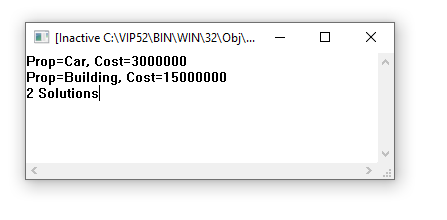
\includegraphics[scale=1]{img/1.png}
    \caption{allProperties(``Ivanov'', ``Moscow'', Prop, Cost).}
\end{figure}

\begin{figure}[H]
    \centering
    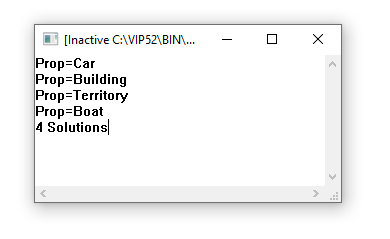
\includegraphics[scale=1]{img/2.png}
    \caption{allProperties(``Ivanov'', ``Saint-Petersburg'', Prop).}
\end{figure}

\begin{figure}[H]
    \centering
    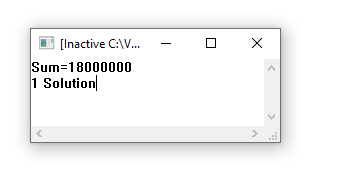
\includegraphics[scale=1]{img/3.png}
    \caption{sumOfCost(``Ivanov'', ``Moscow'', Sum).}
\end{figure}
